% Chapter Template

\chapter{Experimental Setup} % Main chapter title

\label{Chapter3} % Change X to a consecutive number; for referencing this chapter elsewhere, use \ref{ChapterX}

%----------------------------------------------------------------------------------------
%	SECTION 1
%----------------------------------------------------------------------------------------
\section{SPDC Setup}

\begin{figure}[h!]
\centering
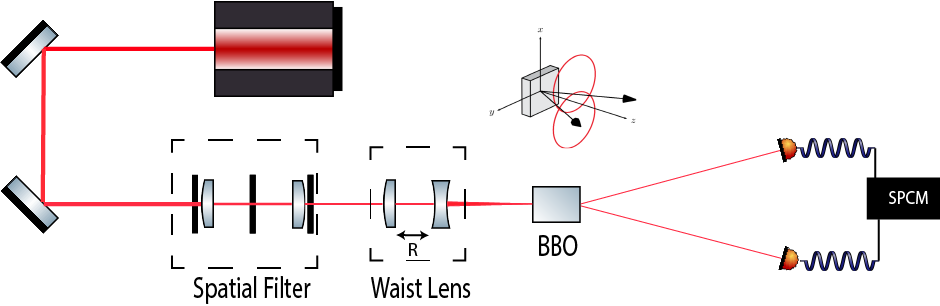
\includegraphics[width=0.65\textwidth]{Figures/SPDC.png}
\caption{Experimental Setup for the SPDC light Source} 
\label{fig:SPDC}
\end{figure}

\subsection{Diode Laser}
The light source used in this experiment is a Diode Laser that delivers a continuous wave(CW) at 
$\lambda = 406,101 nm$ and $\Delta \lambda = 4 nm$. The laser model No. DL 405-200 delivers light at 200 mW with a beam diameter of 1.5 mm and a beam Divergence 1.2 mrad. IN HERE I MAY TALK ABOU THE M FACTOR, QUALITY PARAMETER OF GAUSIAN BEAMS $M^2$ 
Power $200mW$
\begin{figure}[h!]
\centering
{  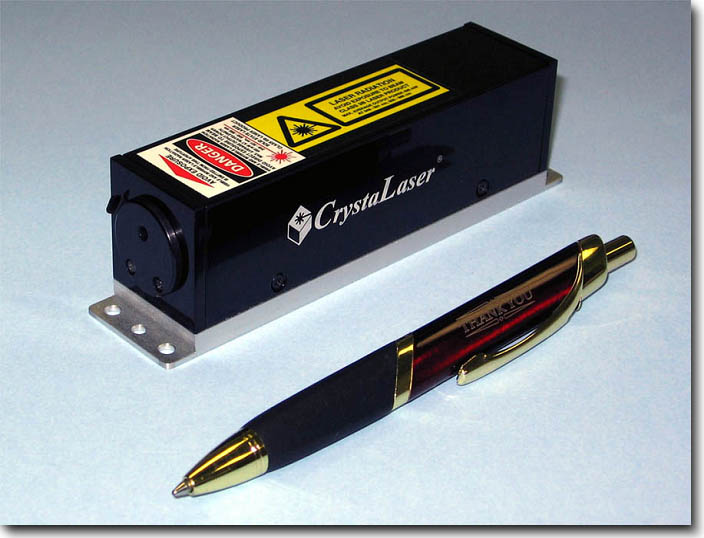
\includegraphics[width=0.5\textwidth]{Figures/diodeLaser.jpg} }
{  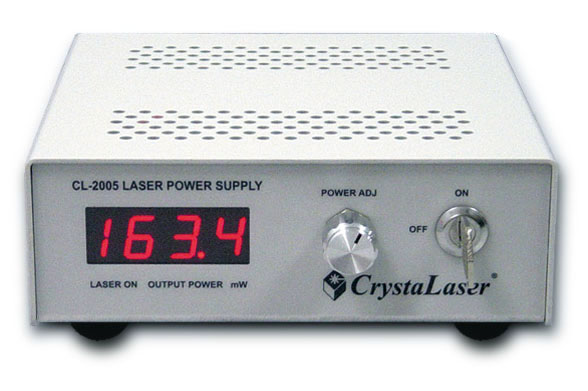
\includegraphics[width=0.5\textwidth]{Figures/diodeLaserControl.jpg} }
\caption{Image of the Diode Laser and it's control module, Taken from \cite{crystalLaser}}
 \label{fig:diodeLaser}
\end{figure}

\subsection{Mirror}
further details to be asked, 
\begin{figure}[h!]
\centering
\label{fig:mirror}
 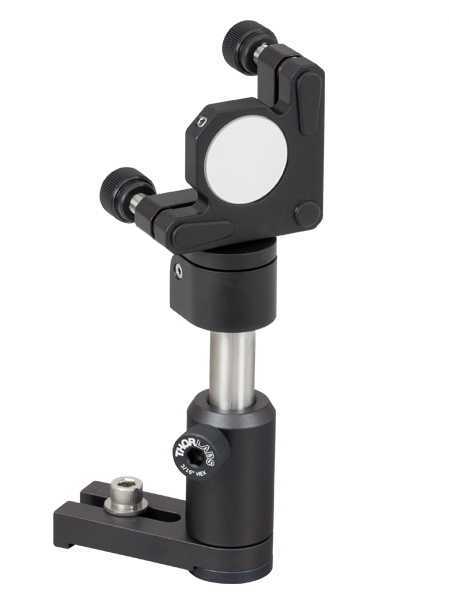
\includegraphics[width=0.45\textwidth]{Figures/mirror.jpg}
 \caption{Mirror and the cavity mount} 
\end{figure}

\subsection{Spatial Filter}
A laser beam can be characterized by measuring its spatial intensity profile at points perpendicular to its direction of propagation. 
The spatial intensity profile is the variation of intensity as a function of distance from the center of the beam, in a plane perpendicular to its direction of propagation.
\begin{figure}[h!]
\centering
{  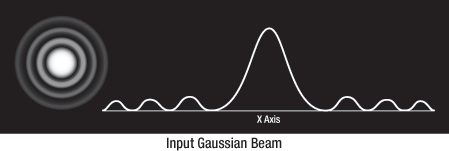
\includegraphics[width=0.55\textwidth]{Figures/inputBeam.png} }
{  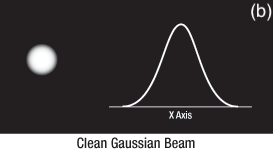
\includegraphics[width=0.55\textwidth]{Figures/outputBeam.png} }
\caption{The spatial intensity profile before and after the spatial filtering process , Taken from \cite{thorlabs}}
 \label{fig:inputOutputBeam}
\end{figure}
In the Figure \ref{fig:inputOutputBeam}(top part) we se see the input gaussian beam 
and how its intensity fluctuates around the x axis. The output desired beam after going through the spatial filter is shown at the bottom 
of the Figure \ref{fig:inputOutputBeam}.
The simplest arrangement to achieve this output spatial intensity profile is show in the Figure \ref{fig:spatialFilter}, 
where at the end we have a beam which intensity strength falls off transversely following a bell-shaped curve that's symmetrical around the central axis.
\begin{figure}[h!]
\centering
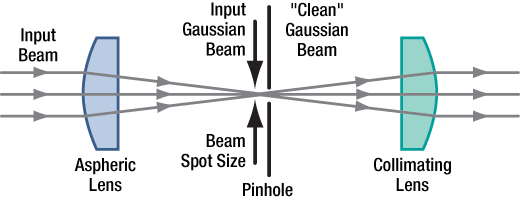
\includegraphics[width=0.55\textwidth]{Figures/spatialFilter.png}
\caption{Basic elements of a Spatial Filter. In our experiment we use a Aspheric Lens of $f=30 mm$(LA1805-A), a pinhole of $50 \mu m$ and a collimating lens of $f=60 mm$(LA1134-A). Taken from \cite{thorlabs}} 
\label{fig:spatialFilter}
\end{figure}
Taking a closer look at the Figure  \ref{fig:inputOutputBeam}(top part) we may recognise a diffraction pattern, but when we measure this spatial profile directly from the diode laser, we find out that it doesn't follow that behaviour, on the contrary 
it follows a more random spatial profile. This ramdom spatial profile is a result of the randomnes in the
quantum emissions and absorptions that are happening at the exited atoms at the diode laser\cite{hecht}.

In order to have this spatial intensity profile at the input of my lens arrangement, Figure \ref{fig:spatialFilter},
we put a circular aperture with the help of a pair of irises, Figure \ref{fig:iris}, before the $f=30.0 mm$ lens and after the $f=60.0mm$ lens.
\begin{figure}[h!]
\centering
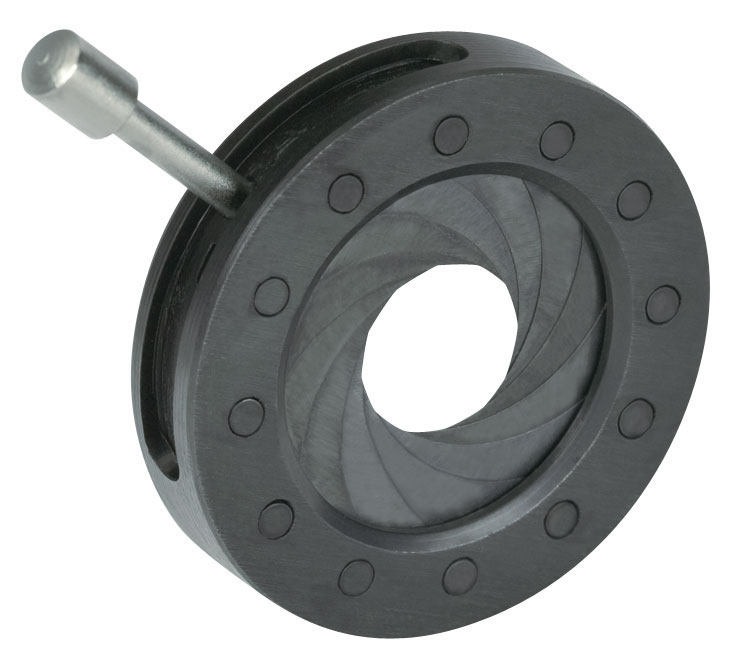
\includegraphics[width=0.25\textwidth]{Figures/iris.jpg}
\caption{This helps to form circular apertures of variable radius} 
\label{fig:iris}
\end{figure}


\subsection{Waist Lens}


\begin{figure}
\centering
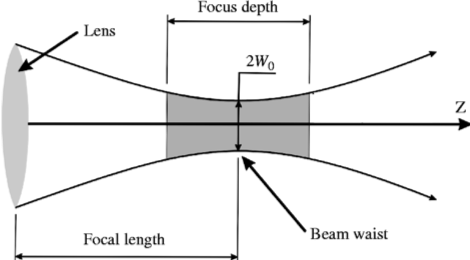
\includegraphics[width=0.35\textwidth]{Figures/waist.png}
\caption{Lens' effect on a Gaussian beam} 
\label{fig:waist}
\end{figure}
A Gaussian beam hits a lens....To control the pump waist we can put a lens in the propagation direction with certain focal lenght $f$. This lens will define a zone around
the distance f called \textit{Focus depth}\cite{hecht} , where in the middle we find the narrowest point of the beam, Figure \ref{fig:waist}.
The radius of this zone is:
\begin{equation}
 W_0=\frac{\lambda f}{\pi W_B}
\end{equation}
Where $W_B$ is the initial waist beam. 
\\
If we want to focus the beam at a fixed distance $F$, using this method to control the pump waist is not practical. 
Every different lens we would use will make this waist $W_0$ at a differents distances $f$. It is necessary to find a \textit{Waist lens}
that make us a waist $W_0$ at a transverse plane located in a fixed position $F$ from the \textit{Waist Lens}. This
special lens consists in an arrangment of two lenses, a positive and negative one respectively, separated a distance 
$d_0$ from each other.
SOURCE WHERE THEY EXPLAIN HOW TO USE A POSITIVE AND NEGATIVE ASK OMAR!!!


\subsection{BBO(Beta Barium Borate) Crystal}

the power of the pump is $60mW$
The nonlinear optical media used in this experiment is a BBO(Beta Barium Borate) crystal, this crystal is $5x5x4 mm$.
BBO (($\beta$-BaB$_{2}$O$_4$)
The crystal is mounted is such way that the input and output plane are fixed, Figure \ref{fig:bbo}.
\begin{figure}
\centering
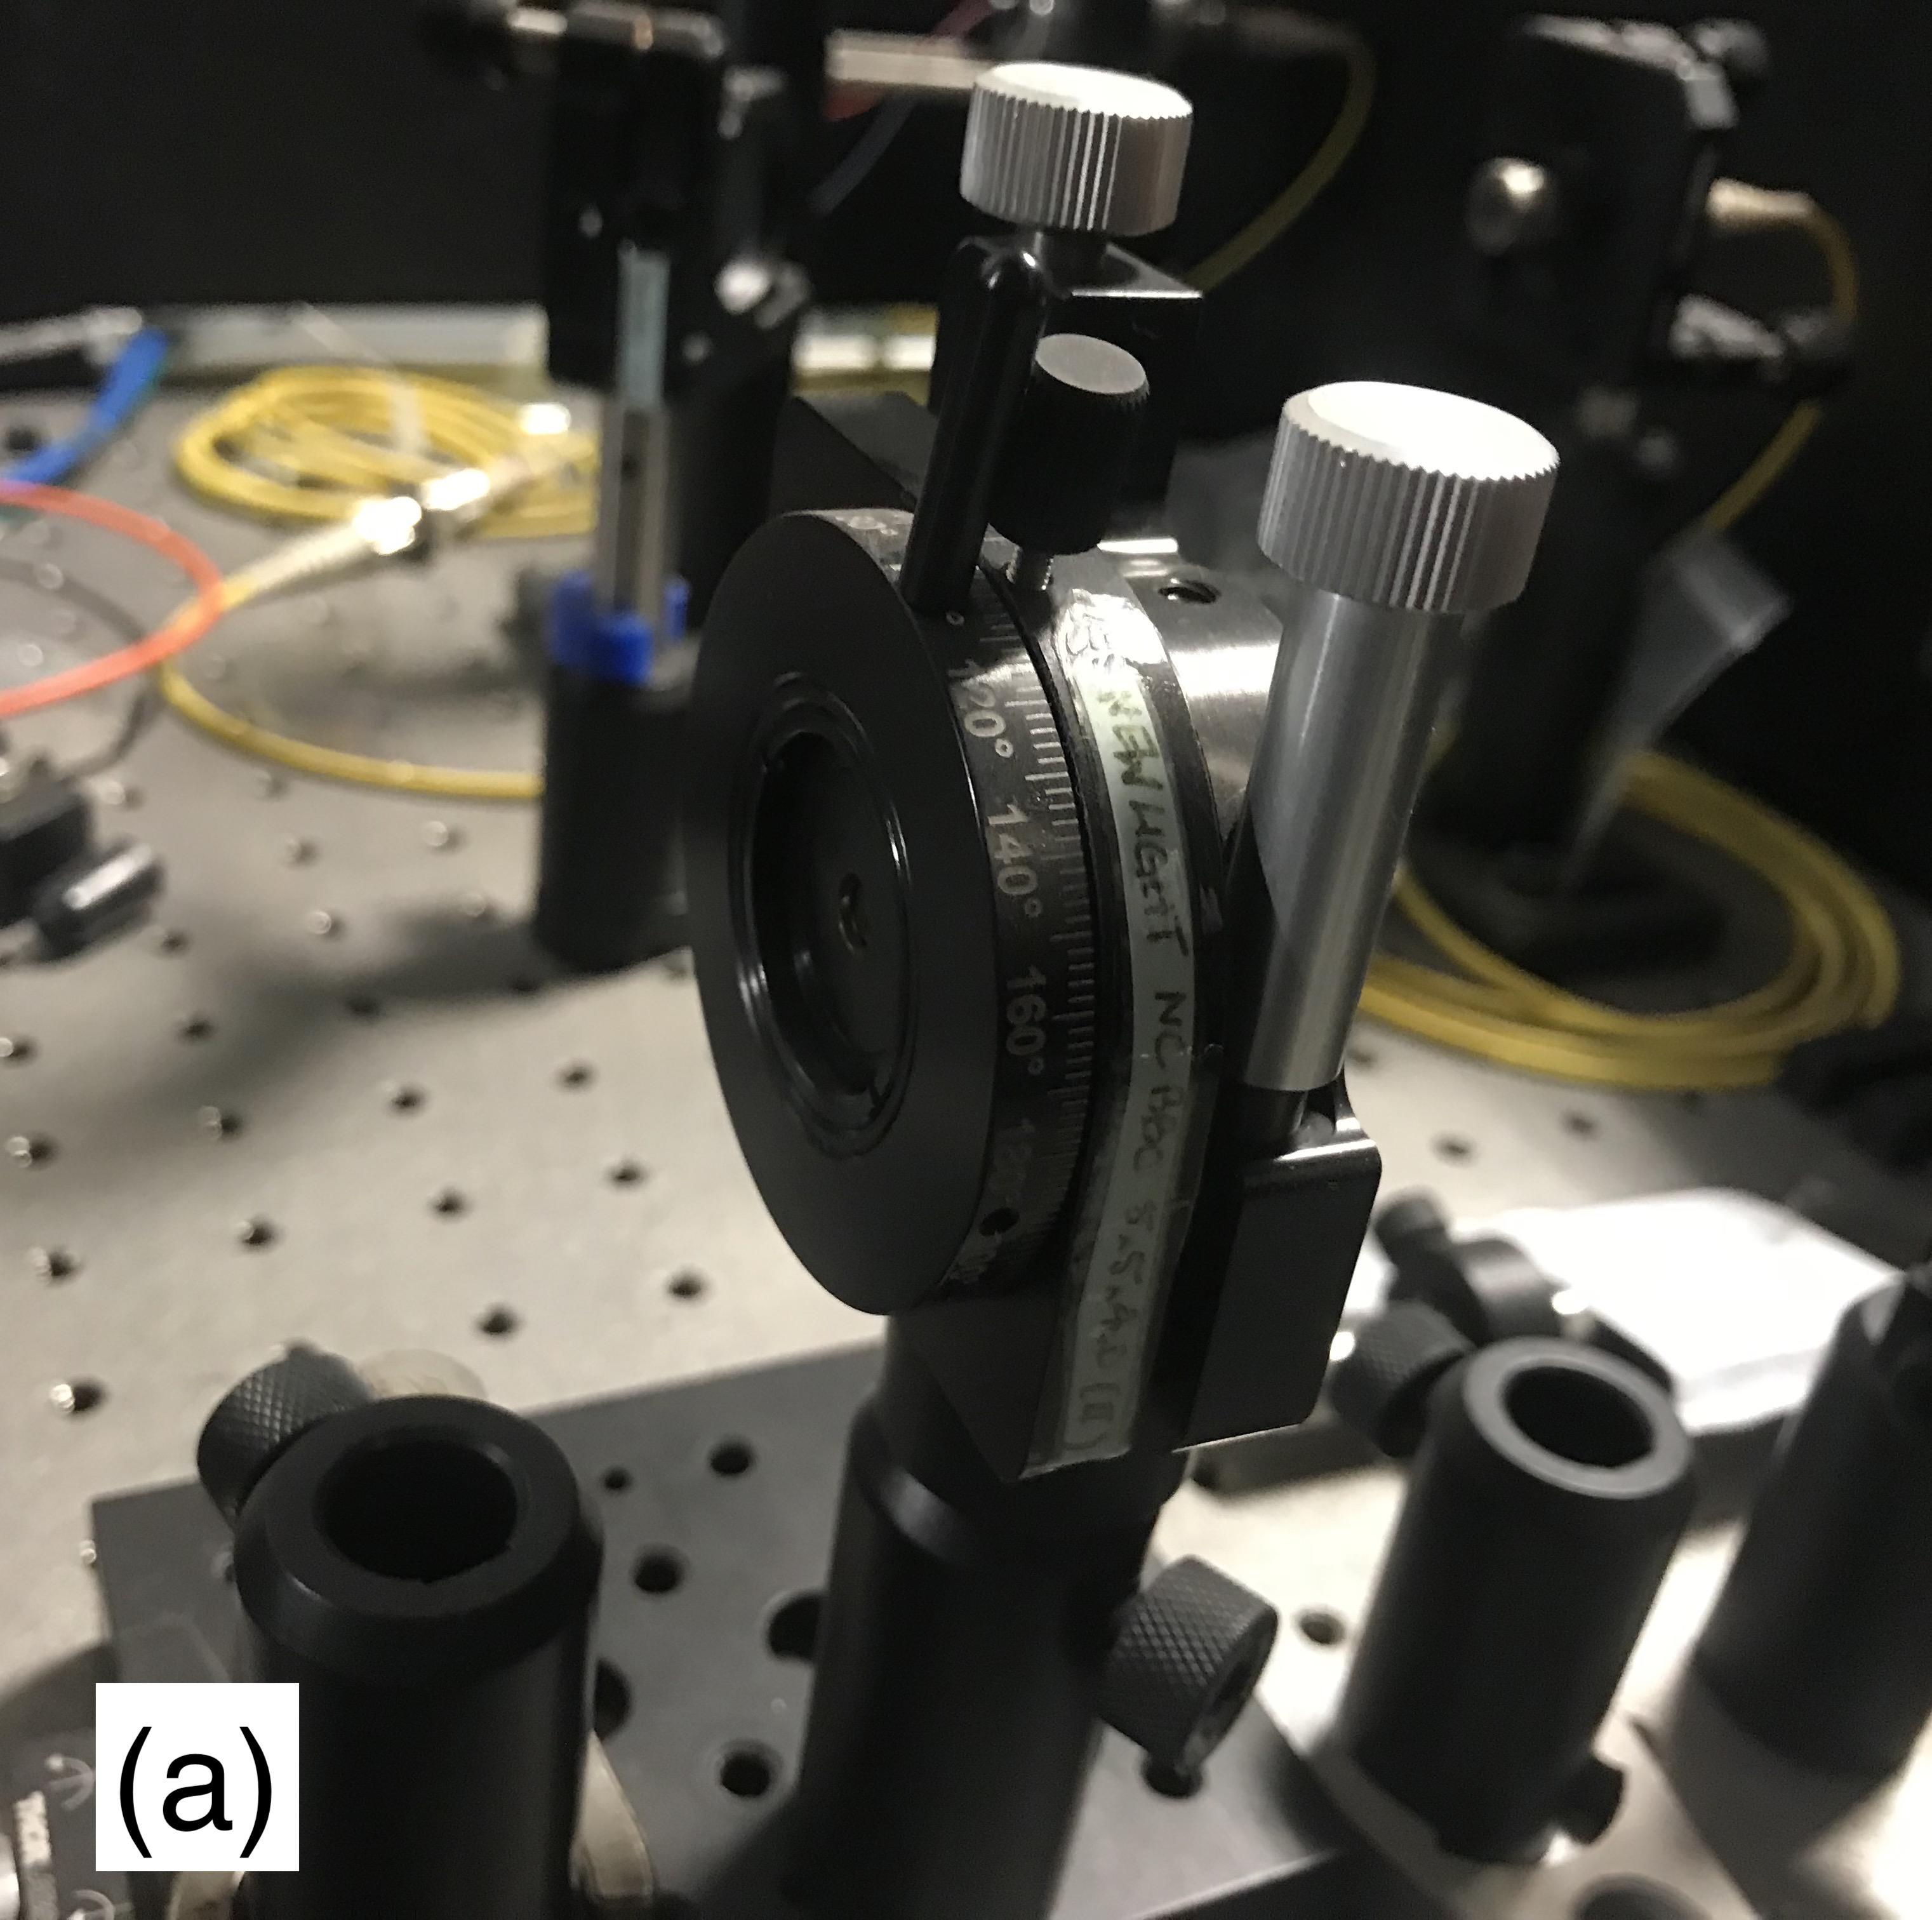
\includegraphics[width=0.35\textwidth]{Figures/bbo.jpg}
\caption{Actual BBO crystal used in experiment} 
\label{fig:bbo}
\end{figure}
 



\section{Spatial Correlations Measurement Setup}
From this point we will talk about a pair of entangled photon pairs, that will come from the output plane of the BBO 
crystal, for historical reasons we will label this pairs as \textit{signal} and \textit{idler}.

\begin{figure}[h!]
\centering
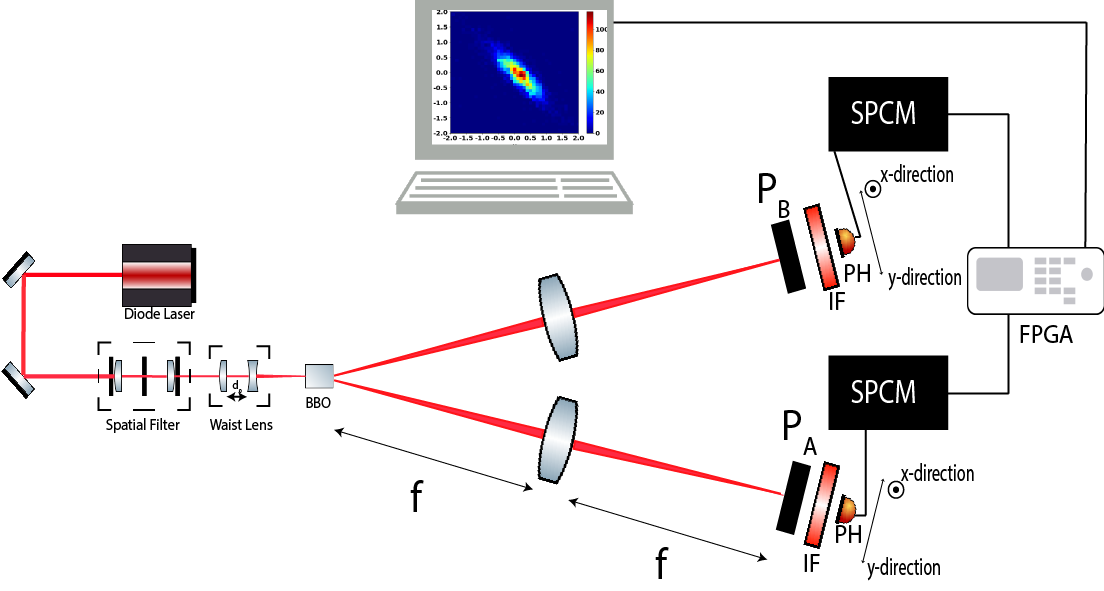
\includegraphics[width=0.75\textwidth]{Figures/spatialCorrelationSetup.png}
\caption{Experimental Setup for Obtaining the spatial correlations of a pair of down-converted photons} 
\label{fig:spatialSetup}
\end{figure}

\subsection{Lens (Fourier Plane)}
To define the $2f$ system we use a lens(LA1708) of $f=200.0mm$ in front of each \textit{signal} and \textit{idler}. 
This lens is placed at a distance $f$ from the output plane.

\subsection{Polariser}
In order to be able to filter certain polarisation direction we used a pair of Polarisers(WP25M-UB), which consist 
in a circular surface than only transmit the light that comes in a specific direction. other directions are reflected

\subsection{Interferometer Filter}
In this situation we are interested in the correlations in the space variables, hence we would like to filter al this 
time variables. To do this filtering we used a spectral filter(FB810-10) that only transmits the light that comes
with $\lambda =810 \pm 2nm$.
\subsection{Pin Hole(Arduino)}
MORE DETAILS, HOW MANY ARDUINOS, coupling lens refernece ETC ...


\subsection{Single Photon Counting Module(SPCM)}
To detect photons we a self-contained module that detects single photons of light over the $400nm$ to $1069 nm$
wavelength range. The module used (SPCM-AQRH-13) uses a unique silicon avalanche photodiode (SLiK) with a detection efficiency of more than 65\%\cite{spcm}.
Light is transmitted through a optic fiber from the pin hole detector to the SPCM. The result signal coming
from the SPCM are pulses that represents one photon detections.
\begin{figure}[h]
\centering
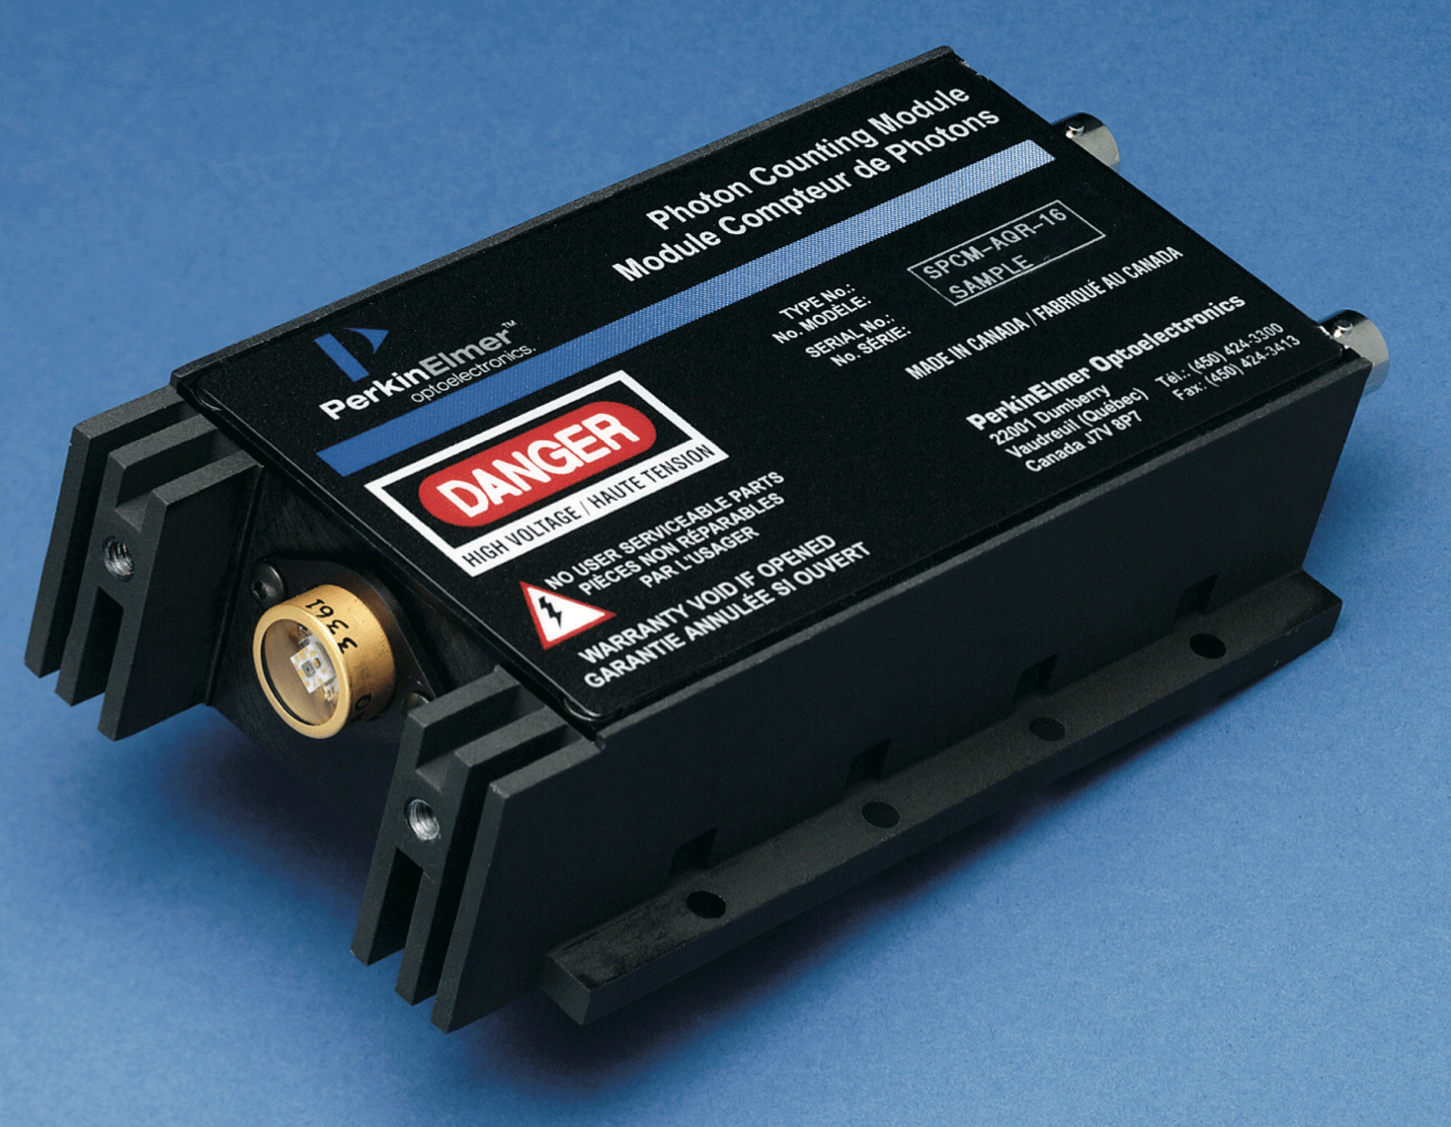
\includegraphics[width=0.35\textwidth]{Figures/spcm.png}
\caption{Single Photon Counting Module} 
\label{fig:spcm}
\end{figure}
\subsection{Field-programmable gate array(FPGA)}
Both \textit{signal} and \textit{idler} pulses from the respective SPCM goes to the same FPGA(ZestSC1). This Field-programmable gate array is programmed
to count the photon coincidences, this means that the FPGA is fast enough to detect and separate pulses from photons 
that are time-separated. 




\subsection{Computer(Data Analysis)}
labview is used to control the detection module, where is delivers a list of the detection, graph are made with any 
program language able to handle the data.


\section{Two-Photon Imaging Setup}
For the Two-photon imaging process we no longer have spatial information about the \textit{signal} photon after it interacts
with the mask  

\begin{figure}[h!]
\centering
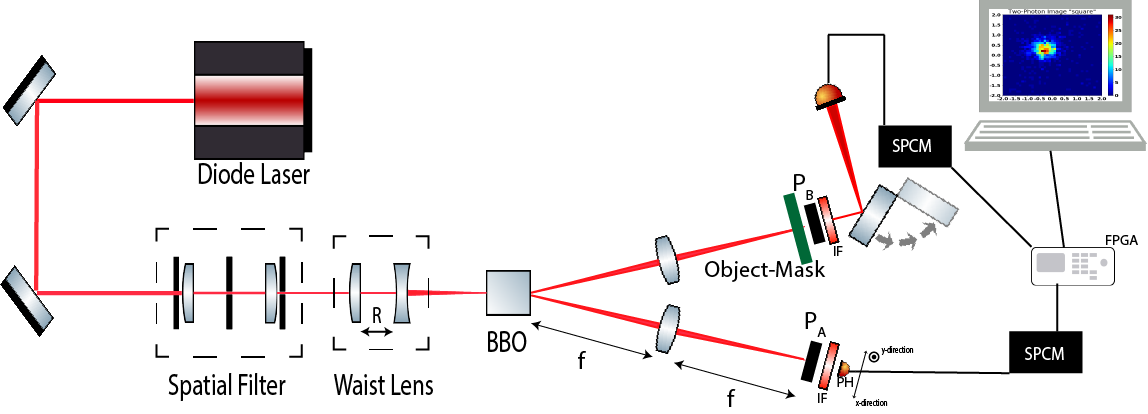
\includegraphics[width=0.75\textwidth]{Figures/ghostSetup.png}
\caption{Experimental Setup for the Two-photon Imaging} 
\label{fig:ghostSetup}
\end{figure}

\subsection{Mask}
This is an obstruction that is placed in the \textit{signal} path with certain shape, it could be a mask with the shape of a letter or any other geometry. This is the object 
of which we want to construct an image.
\subsection{Folding Mirror}
In order to change de path followed by the \textit{signal} photon, we use a Folding mirror, Figure \ref{fig:foldingMirror}.
This mirror can be in the \textit{signal} path or not.
\begin{figure}[h]
\centering
 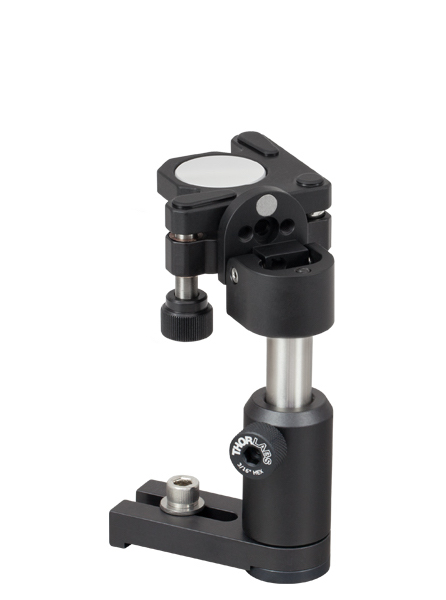
\includegraphics[width=0.25\textwidth]{Figures/foldingMirror.jpg}
 \caption{Foldind Mirror, it is in the position for measuring the correlations}
\label{fig:foldingMirror} 
\end{figure}

\subsection{Bucket Detector}
This detector consist in a coupling lens that collects all the light that goes through the mask, 
In contrast to the other detections made in this experiment, the Bucket detector loses track of any spatial information of the \textit{signal} photon. Another big difference is that this Bucket detector uses a multimode optic fiber to take the light to the SPCM.

